\documentclass{article}
\usepackage{graphicx}
\usepackage{amsmath}
\usepackage{caption}
\usepackage{float}

\title{Labwork 2: Linear Regression Using Gradient Descent}
\author{Le Duc Bach - ICT.2440039}
\date{}

\begin{document}

\maketitle

\section{Introduction}
Linear regression is a statistical method used to model the relationship between a dependent variable and one or more independent variables. This lab demonstrates how to implement simple linear regression using gradient descent to minimize the mean squared error (MSE) between the predicted and actual values.

\section{Methodology}
\subsection*{Dataset}
The dataset used is a CSV file (\texttt{lr.csv}) containing two columns representing the independent variable ($x$) and the dependent variable ($y$).

\subsection*{Loss Function}
The loss function is defined as:
\[
f(w_0, w_1, x_i, y_i) = \frac{1}{2}(w_1 x_i + w_0 - y_i)^2
\]
The objective is to minimize the average loss over all data points.

\subsection*{Gradient Calculation}
The gradients with respect to $w_0$ and $w_1$ are:
\[
\frac{\partial f}{\partial w_0} = w_1 x_i + w_0 - y_i
\]
\[
\frac{\partial f}{\partial w_1} = x_i(w_1 x_i + w_0 - y_i)
\]

\subsection*{Gradient Descent Update}
We update the parameters as follows:
\[
w_0 := w_0 - \alpha \cdot \frac{1}{N} \sum_{i=1}^{N} \frac{\partial f}{\partial w_0}
\]
\[
w_1 := w_1 - \alpha \cdot \frac{1}{N} \sum_{i=1}^{N} \frac{\partial f}{\partial w_1}
\]
where $\alpha$ is the learning rate, and $N$ is the number of data points.

\section{Implementation}
The implementation was done in Python using \texttt{matplotlib} for visualization. The model was trained for 200 iterations with a learning rate of 0.001.

\section{Results}
\begin{figure}[H]
    \centering
    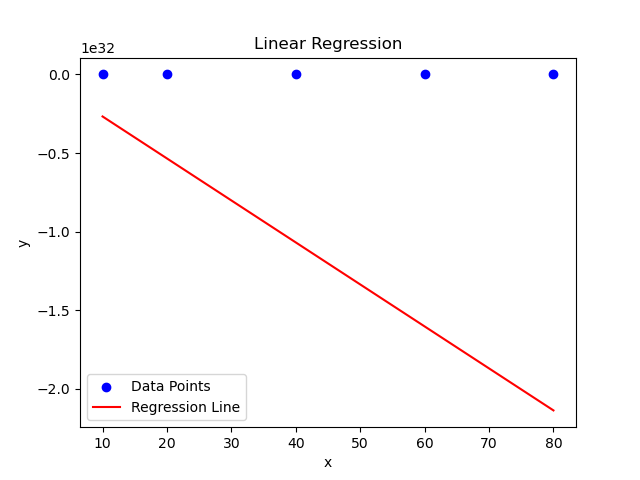
\includegraphics[width=0.8\textwidth]{Figure_1.png}
    \caption{Linear regression fit after training}
\end{figure}

\begin{figure}[H]
    \centering
    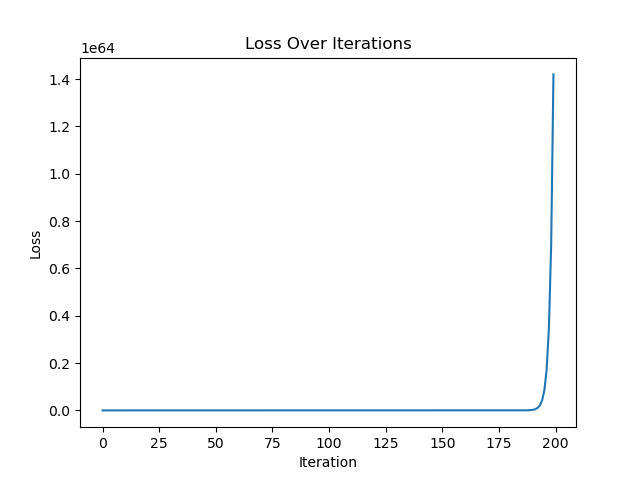
\includegraphics[width=0.8\textwidth]{Figure_2.png}
    \caption{Loss over 200 iterations of gradient descent}
\end{figure}

The plot shows that the loss increases exponentially, indicating that the learning rate may be too high, causing divergence instead of convergence. As a result, the regression line does not fit the data properly.

\section{Conclusion}
This lab highlights the importance of choosing an appropriate learning rate for gradient descent. Even though the implementation was correct, the poor choice of learning rate led to divergence in the loss function and an inaccurate regression line. Future improvements could involve tuning hyperparameters or implementing learning rate decay.

\end{document}
